\documentclass[a4paper,11pt]{article}
\usepackage{amsmath, bm}
\usepackage{amssymb,amsthm,graphicx}
\usepackage{enumitem}
\usepackage{color}
\usepackage{epsfig}
\usepackage{graphics}
\usepackage{pdfpages}
\usepackage{subcaption}
\usepackage[font=small]{caption}
\usepackage[hang,flushmargin]{footmisc} 
\usepackage{float}
\usepackage{rotating,tabularx}
\usepackage{booktabs}
\usepackage[mathscr]{euscript}
\usepackage{natbib}
\usepackage{setspace}
\usepackage{placeins}
\usepackage{ulem}
\usepackage[left=3cm,right=3cm,bottom=3cm,top=3cm]{geometry}
\numberwithin{equation}{section}
\allowdisplaybreaks[3]


% General

\newcommand{\reals}{\mathbb{R}}
\newcommand{\integers}{\mathbb{Z}}
\newcommand{\naturals}{\mathbb{N}}

\newcommand{\pr}{\mathbb{P}}        % probability
\newcommand{\ex}{\mathbb{E}}        % expectation
\newcommand{\var}{\textnormal{Var}} % variance
\newcommand{\cov}{\textnormal{Cov}} % covariance

\newcommand{\law}{\mathcal{L}} % law of X
\newcommand{\normal}{N}        % normal distribution 

\newcommand{\argmax}{\textnormal{argmax}}
\newcommand{\argmin}{\textnormal{argmin}}

\newcommand{\ind}{\mathbbm{1}} % indicator function
\newcommand{\kernel}{K} % kernel function
\newcommand{\wght}{W} % kernel weight
\newcommand{\thres}{\pi} % threshold parameter


% Convergence

\newcommand{\convd}{\stackrel{d}{\longrightarrow}}              % convergence in distribution
\newcommand{\convp}{\stackrel{P}{\longrightarrow}}              % convergence in probability
\newcommand{\convas}{\stackrel{\textrm{a.s.}}{\longrightarrow}} % convergence almost surely
\newcommand{\convw}{\rightsquigarrow}                           % weak convergence


% Theorem-like declarations

\theoremstyle{plain}

\newtheorem{theorem}{Theorem}[section]
\newtheorem{prop}[theorem]{Proposition}
\newtheorem{lemma}[theorem]{Lemma}
\newtheorem{corollary}[theorem]{Corollary}
\newtheorem*{theo}{Theorem}
\newtheorem{propA}{Proposition}[section]
\newtheorem{lemmaA}[propA]{Lemma}
\newtheorem{definition}{Definition}[section]
\newtheorem{remark}{Remark}[section]
\renewcommand{\thelemmaA}{A.\arabic{lemmaA}}
\renewcommand{\thepropA}{A.\arabic{propA}}
\newtheorem*{algo}{Clustering Algorithm}


% Theorem numbering to the left

\makeatletter
\newcommand{\lefteqno}{\let\veqno\@@leqno}
\makeatother


% Heading

\newcommand{\heading}[2]
{  \setcounter{page}{1}
   \begin{center}

   \phantom{Distance to upper boundary}
   \vspace{0.5cm}

   {\LARGE \textbf{#1}}
   \vspace{0.4cm}
 
   {\LARGE \textbf{#2}}
   \end{center}
}


% Authors

\newcommand{\authors}[4]
{  \parindent0pt
   \begin{center}
      \begin{minipage}[c][2cm][c]{5cm}
      \begin{center} 
      {\large #1} 
      \vspace{0.05cm}
      
      #2 
      \end{center}
      \end{minipage}
      \begin{minipage}[c][2cm][c]{5cm}
      \begin{center} 
      {\large #3}
      \vspace{0.05cm}

      #4 
      \end{center}
      \end{minipage}
   \end{center}
}

%\newcommand{\authors}[2]
%{  \parindent0pt
%   \begin{center}
%   {\large #1} 
%   \vspace{0.1cm}
%      
%   #2 
%   \end{center}  
%}


% Version

\newcommand{\version}[1]
{  \begin{center}
   {\large #1}
   \end{center}
   \vspace{3pt}
} 










\begin{document}



\heading{Clustering of the epidemic time trends:}{the case of COVID-19}

%\authors{Marina Khismatullina\renewcommand{\thefootnote}{1}\footnotemark[1]}{University of Bonn}{Michael Vogt\renewcommand{\thefootnote}{2}\footnotemark[2]}{Ulm University} 
%\footnotetext[1]{Corresponding author. Address: Bonn Graduate School of Economics, University of Bonn, 53113 Bonn, Germany. Email: \texttt{marina.k@uni-bonn.de}.}
%\renewcommand{\thefootnote}{2}
%\footnotetext[2]{Address: Institute of Statistics, Department of Mathematics and Economics, Ulm University, 89081 Ulm, Germany. Email: \texttt{m.vogt@uni-ulm.de}.}
%\renewcommand{\thefootnote}{\arabic{footnote}}
%\setcounter{footnote}{2}

%\vspace{-0.85cm}

%\renewcommand{\baselinestretch}{1.2}\normalsize

%\renewcommand{\abstractname}{}
%\begin{abstract}
%\noindent The COVID-19 pandemic is one of the most pressing issues at present. A question which is particularly important for governments and policy makers is the following: Does the virus spread in the same way in different countries? Or are there significant differences in the development of the epidemic? In this paper, we devise new inference methods that allow to detect differences in the development of the COVID-19 epidemic across countries in a statistically rigorous way. In our empirical study, we use the methods to compare the outbreak patterns of the epidemic in a number of European countries.
%\end{abstract}

%\noindent \textbf{Key words:} simultaneous hypothesis testing; multiscale test; time trend; panel data; COVID-19.

%\noindent \textbf{JEL classifications:} C12; C23; C54.

%\noindent \textbf{AMS 2010 subject classifications:} 62E20; 62G10; 62G15; 62G20.

\renewcommand{\baselinestretch}{1.5}\normalsize



\section{Model}

Suppose we observe a large number of time series $\mathcal{Y}_i = \{Y_{it}: 1 \leq t \leq T\}$ for $1 \leq i \leq n$ and each time series $\mathcal{Y}_i$ satisfies the following nonparametric regression equation
\begin{equation}\label{eq:model}
Y_{it} = m_i\Big(\frac{t}{T}\Big) + u_{it}
\end{equation}
for $t \in \{1, \ldots, T\}$ with $m_i(\cdot)$ being an unknown smooth function defined on $[0, 1]$. As usual in nonparametric regression \citep[see e.g.][]{Robinson1989}, we let the regression function $m_i$ in model \eqref{eq:model} depend on rescaled time $t/T$ rather than on real time $t$. The assumptions for the error term $u_{it}$ will be discussed later.

Suppose that all of the unknown functions $m_i(\cdot)$ can be divided into $K$ classes in the following way:
\begin{itemize}
	\item Each of the $K$ classes of functions $\class_k$ are defined as\\
	 $\mathcal{F}_k := \{ f:[0, 1] \rightarrow R \,|\, f = c \cdot g_k(b \cdot u)$ with $c>0, b\in [1, \bar{b}]$ and $g_k$ a density function$\}$.\\
	 We assume that $\bar{b}$ is known beforehand. For the identification purposes, we also assume that the classes are distinct, i.e. $\class_k \cap \class_{k^\prime} = \empty$ for any $k \neq k^\prime$. 
	 \item Suppose that $\{1, \ldots, n\} = \cup_{k=1}^k \mathcal{G}_k$ such that for any $k$ we have
	 \vspace{-2mm}
	 $$m_i \in \class_k \text{ for all } i \in \mathcal{G}_k.$$
	In other words, for all $i \in \{1, \ldots, n\}$ we can write $m_i(u) = c \cdot g_k (b \cdot u)$ for some $k \in \{1, \ldots, K\}$, $c > 0 $ and $b \in [1, \bar{b}]$.
\end{itemize} 

We can regard $c$ as the country-specific scaling parameter that accounts for the size of the country or population density. We introduce this additional parameter in order to be able to compare countries that differ substantially in terms of the population, i.e. Luxembourg and Russia. We can regard $b$ as a time parameter that is responsible for the speed of the development of the pandemic. If we compare two countries $i$ and $j$  that belong to the same class $k$ but have different time parameters, $b_i$ and $b_j$ respectively, and $b_i > b_j$, then we can say that country $i$ experiences a more rapid development of the pandemic relative to country $j$ even though the general shapes of the regression functions $m_i$ and $m_j$ are the same.

In what follows, we present a method that allows researchers to discover the group structure of the time trends of new COVID-19 cases in different countries and to cluster the countries based on the shape of the respective regression functions.

%For the identification purposes, we need to assume that for each $i \in \mathcal{C}$ we have $\int_0^1 \lambda_i(u)du = 1$. Only then we are able to estimate the scaling parameter $c_i$. Thus, the testing procedure is as follows.

\section{Clustering procedure}

Let $i$ and $j$ be two countries from our sample. In this subsection we construct a dissimilarity measure $\widehat{\Delta}_{ij}$ that estimates how far the functions $m_i$ and $m_j$ are from each other. This dissimilarity measure $\widehat{\Delta}_{ij}$ will serve as a distance measure between the functions $m_i$ and $m_j$ in our clustering algorithm later on.

\textit{Step 1}

First, for each $i$ we nonparametrically estimate $m_i(u)$ using Nadaraya-Watson estimation procedure with a rectangular kernel and a bandwidth window that covers $7$ data points, i.e. $7$ days. This choice of a bandwidth allows us to take care of possible weekly cycles in the data which are produced by delays in reporting new cases over the weekend. As a robustness check, we repeat our analysis for the multiples of $7$ days, i.e. for bandwidth windows covering $14$ and $21$ days. We report the results of the robustness checks in the Supplementary Material.

Formally, the estimator $\hat{m}_i$ estimated at $u\in [0, 1]$ is defined as
$$\hat{m}_i(u) = \sum_{t=1}^T \frac{K_h(u - t/T) Y_{it}}{\sum_{s=1}^T K_h(u - s/T)}$$
with $K_h(u - t/T)$ being a rectangular kernel: $K_h(x) = \frac{1}{2}$ for $|x| \leq h$ and $K_h(x) = 0$ otherwise.

\textit{Step 2}

Second, for a given value of $b \in [1, \bar{b}]$ and for a given pair of countries $(i, j)$, consider the following statistic:
\begin{align*}
	\delta_{ij}(b) = \frac{1}{1/b} \int_0^{1/b} \bigg( \frac{\hat{m}_i (b\cdot u)}{\int_0^{1/b} \hat{m}_i(b\cdot v) dv /(1/b)}  - \frac{\hat{m}_j (u)}{\int_0^{1/b} \hat{m}_j(v) dv /(1/b)}  \bigg)^2 du.
\end{align*}
$\delta_{ij}(b)$ can be regarded as a measure of dissimilarity between $m_i(b \cdot u)$ and $m_j(u)$ on an interval $[0, 1/b]$ for a specific value of $b$. Note that generally speaking $\delta_{ij}(b) \neq \delta_{ji}(b)$ for $i \neq j$.

%Suppose that countries $i$ and $j$ belong to the same class $\mathcal{G}_k$, i.e. $m_i(u) = c_i g_k (b_i u)$ and $m_j(u) = c_j g_k(b_j u)$. Without loss of generality, assume that $b_i \geq b_j$.  Since $Y_{it} = m_i(t/T) + u_{it}$, we can rewrite the estimators $\hat{m}_i$  as follows: 
%\begin{align*}
%\hat{m}_i(u) &= \sum_{t=1}^T \frac{K_h(u - t/T) (m_i(t/T) + u_{it})}{\sum_{s=1}^T K_h(u - s/T)} \\
%&= \sum_{t=1}^T \frac{K_h(u - t/T) (c_i g_k (b_i \cdot t/T) + u_{it})}{\sum_{s=1}^T K_h(u - s/T)}\\
%&=c_i  \sum_{t=1}^T \frac{K_h(u - t/T) g_k (b_i \cdot t/T)}{\sum_{s=1}^T K_h(u - s/T)} + \sum_{t=1}^T \frac{K_h(u - t/T) u_{it}}{\sum_{s=1}^T K_h(u - s/T)}
%\end{align*}


%Then for $b = b_i/b_j$ we have $m_i(u)/c_i = m_j(b u)/c_j$.

\textit{Step 3}

We now construct a dissimilarity measure between two countries $i$ and $j$ that does not depend on a specific choice of a time parameter $b$. In order to do so, we would like to aggregate $\delta_{ij}(b)$ for different values of $b$. %According to the reasons stated above, 
If the functions $m_i$ and $m_j$ belong to the same class, then for some $b_0\in [1, \bar{b}]$ we will have $\delta_{ij}(b_0)$ close to zero. \textcolor{red}{Need to show that!} Hence, we aggregate the measures $\delta_{ij} (b)$ by taking the infimum over all possible values of $b$:
\begin{align*}
	\widehat{\Delta}_{ij} = \min \{ \inf_{b\in [1, \bar{b}]} \delta_{ij}(b), \inf_{b\in [1, \bar{b}]} \delta_{ji}(b) \}
\end{align*}

\textit{Step 4}

Based on $\widehat{\Delta}_{ij}$, we run a hierarchical agglomerative clustering (HAC) algorithm using complete linkage criterion. Detailed description of the algorithm and its properties are presented in Section \ref{sec:alg}.

\section{Clustering algorithm}\label{sec:alg}

Let $S \subseteq \{1, \ldots, n\}$ and $S^\prime \subseteq \{1, \ldots, n\}$ be two sets of time series from our sample. There are several ways to define a dissimilarity measure between $S$ and $S^\prime$. In our paper, we work with the complete linkage measure of dissimilarity defined as 
\begin{align*}
\Delta (S, S^\prime) = \max_{i \in S, j\in S^\prime} \widehat{\Delta}_{ij}.
\end{align*}
Alternatively, we may use single or average linkage measure 

{\color{red} This description I copied from your paper.

To partition the set of time series $\{1,\ldots, n\}$ into groups, we combine the dissimilarity measure $\Delta$ with a HAC algorithm which proceeds as follows:

\textbf{Algorithm} (HAC Algorithm).

\textit{Step 0 (Initialization):} Let $\hat{G}_i^{[0]} = \{i\}$ denote the $i$th singleton cluster for $1 \leq i \leq n$ and define $\{\hat{G}_1^{[0]}, \ldots, \hat{G}_n^{[0]}\}$ to be the
initial partition of time series into clusters.

\textit{Step r (Iteration):} Let $\hat{G}^{[r-1]}_1, \ldots, \hat{G}^{[r-1]}_{n - (r-1)}\}$ be the $n-(r-1)$ clusters from the previous step. Determine the pair of clusters $\hat{G}^{[r-1]}_k$ and $\hat{G}^{[r-1]}_{k^\prime}$ for which 
\begin{align*}
\Delta(\hat{G}^{[r-1]}_{k}, \hat{G}^{[r-1]}_{k^\prime}) = \min_{1 \leq l < l^\prime \leq n- (r-1)} \Delta(\hat{G}^{[r-1]}_{l}, \hat{G}^{[r-1]}_{l^\prime})
\end{align*}
and merge them into a new cluster.

Iterating this procedure for $r = 1, \ldots, n-1$ yields a tree of nested partitions \linebreak $\{\hat{G}^{[r]}_1, \ldots, \hat{G}^{[r]}_{n-r} \}$, which can be graphically
represented by a dendrogram. Roughly speaking, the HAC algorithm merges the n singleton clusters $\hat{G}^{[0]}_i = \{i\}$ step by step until we end up with the cluster $\{1, \ldots, n\}$. In each step of the algorithm, the closest two clusters are merged, where the distance between clusters is measured in terms of the dissimilarity $\Delta$ We refer the reader to \cite{Ward1963} for an early reference on HAC clustering and to Section 14.3.12 in \cite{HastieTibshiraniFriedman2009} for an overview of hierarchical clustering methods.}

\section{Application}\label{sec:app}

We now use our clustering procedure to analyze the outbreak patterns of the COVID-19 epidemic. We proceed in two steps. In Section \ref{subsec:sim}, we assess the finite sample performance of our method by Monte-Carlo experiments. In Section \ref{subsec:app}, we apply the method to a sample of COVID-19 data for $104$ different countries.

\subsection{Simulation}\label{subsec:sim}

\subsection{Analysis of the COVID-19 data}\label{subsec:app}

\subsubsection{Data}


We analyze data from $104$ countries. We chose only those countries that have a total number of not less than $20\,000$ cases of infection during the considered time period. For each country $i$, we observe a time series $\mathcal{Y}_i = \{ Y_{it}: 1 \le t \le T \}$, where $Y_{it}$ is the number of newly confirmed COVID-19 cases in country $i$ on day $t$. The data are freely available on the homepage of the European Center for Disease Prevention and Control (\texttt{https://www.ecdc.europa.eu}) and were downloaded on 25 February 2021.\footnote{ECDC switched to a weekly reporting schedule for the COVID-19 situation on 17 December 2020. Hence, all daily updates have been discontinued from 14 December. The downloaded daily data set presents historical data until 14 December 2020.} As already mentioned in the Introduction, we take the first Monday after reaching $100$ confirmed cases in each country as the starting date $t=1$. Beginning the time series of each country on the day when that country reached $100$ confirmed cases is a common way of ``normalizing'' the data \citep[see e.g.][]{Cohen2020}. Additionally aligning the data by Monday allows to take care of possible weekly cycles in the data which are produced by delays in reporting new cases over the weekend. The time series length $T$ is taken to be the longest interval for which we have observations for all $104$ countries. The resulting dataset thus consists of $n = 104$ time series, each with $T = 192$ observations. Some of the time series contain negative values which we replaced by $0$. Overall, this resulted in $14$ replacements.

We assume that the data $Y_{it}$ of each country $i$ in our sample follow the nonparametric trend model 
\[ Y_{it} = m_i\Big(\frac{t}{T}\Big) + u_{it}, \]
which was introduced in equation \eqref{eq:model}. As in the theoretical part of the paper, we assume that all of the countries $i$ can be partitioned into $K$ classes $\mathcal{G}_1, \ldots, \mathcal{G}_K$ such that for each $1 \leq k\leq K$ and for all $i \in \mathcal{G}_k$, $m_i(u) = c \cdot g_k(b \cdot u)$ for some $c>0$ and $b\in[1, \bar{b}]$. We thus suppose that the general shape of the time trends $m_i$ are the same (or at least very similar) in all countries $i$ in a given group $\mathcal{G}_k$, but the scale and time parameters may vary across countries from the same group. We take $\bar{b} = 2$ which is more than enough for our purposes. Note that $\bar{b}$ accounts for the largest value of the time parameter, and allowing for some countries to be twice as fast as some others is already a very generous assumption.

Throughout the section, we set implement the clustering procedure in exactly the same way as in the simulation study of Section \ref{subsec:sim}. In particular, we use a rectangular kernel $K_h$ to compute the local linear smoothers $\hat{m}_{i}$ and consider the bandwidth $h = 3.5/T$, which corresponds to an effective sample size of $7$ days of data. Moreover, we assume that the number of classes $K$ is equal to $7$.

Furthermore, the values $\delta_{ij}(b)$ and $\delta_{ji}(b)$ are calculated not for all $b\in [1, \bar{b}]$, but on a grid that consists of the values $\{1, 1.01, 1.02, \ldots, \bar{b}\}$. Since this grid is finite, in what follows we will be working with $\min_{b \in [1, \bar{b}]} \delta_{ij}(b)$ and $\min_{b \in [1, \bar{b}]} \delta_{ji}(b)$ instead of $\inf_{b \in [1, \bar{b}]} \delta_{ij}(b)$ and $\inf_{b \in [1, \bar{b}]} \delta_{ji}(b)$.

The results of our algorithm are presented in Figures \ref{fig:dend} - \ref{fig:map}. First, Figure \ref{fig:dend} presents the corresponding dendrogram of a HAC. Different colours of the countries correspond to the different classes they belong to (by our clustering algorithm). Then, Figures \ref{fig:cl1} - \ref{fig:cl7} present the trend functions of the countries that belong to the group $\mathcal{G}_1, \ldots, \mathcal{G}_6$ respectively. For comparability reasons, instead of plotting $\hat{m}_i(u)$, we opted for plotting $\hat{m}_i(\hat{b}_i \cdot u) / \hat{c}_i$ where $\hat{b}_i$ and $\hat{c}_i$ are computed according to \eqref{eq:b_hat} and \eqref{eq:c_hat} in the algorithm described below.

\newpage
\textit{Step 1}

First, define the following quantities:
\begin{align*}
b_{ij} &= \begin{cases}
\arg \min_{b \in [1, \bar{b}]} \delta_{ij}(b),  &\text{ if } \min_{b \in [1, \bar{b}]} \delta_{ij}(b) \leq \min_{b \in [1, \bar{b}]} \delta_{ji}(b), \\
1, &\text{ otherwise};
\end{cases}\\
 \text{ and } b_{ji} &=\begin{cases}
\arg \min_{b \in [1, \bar{b}]} \delta_{ji}(b),  &\text{ if } \min_{b \in [1, \bar{b}]} \delta_{ji}(b) < \min_{b \in [1, \bar{b}]} \delta_{ij}(b), \\
1, &\text{ otherwise}.
\end{cases}
\end{align*}
The idea behind these values is that our algorithm estimates the dissimilarity measure between countries $i$ and $j$ to be the smallest when their respective time parameters are equal to $b_{ij}$ and $b_{ji}$. These quantities are calculated for all pairs $i$ and $j$ irrespective of countries $i$ and $j$ being in the same class. However, if the countries $i$ and $j$ are indeed in the same class $k$, we have that $m_i(u) = c_i \cdot g_k (b_i \cdot u)$ and $m_j(u) = c_j \cdot g_k( b_j \cdot u)$. Hence,
$$m_i \Big( \frac{u}{b_i} \Big) / c_i= g_k (u) = m_j \Big( \frac{u}{b_j} \Big) /c_j,$$
and thus,
$$m_i (u) / c_i = m_j \Big( \frac{b_i}{b_j} u \Big) /c_j,$$
or, alternatively,
$$m_i\Big( \frac{b_j}{b_i} u \Big) /c_i = m_j (u) / c_j$$
If $b_i \geq b_j$, then $b_{ji}$ can be regarded as an approximation of $b_i / b_j$ (and $b_{ij}$ should be equal to $1$), and if $b_i < b_j$, then $b_{ij}$ can be regarded as an approximation of $b_j/b_i$ (and $b_{ji}$ should be equal to $1$). In any case, $m_i( b_{ij} u ) /c_i \approx m_j (b_{ji} u) / c_j$.

\textit{Step 2}

Using the quantities from Step 1, we pick a representative time series $i_k$ for each cluster $k$. If the cluster $k$ consists only of one element, then the representative time series should be the only member of the cluster. This is, for example, the case for clusters $6$ and $7$ (see Figures \ref{fig:cl6} and \ref{fig:cl7}). However, if the number of elements in a cluster is greater than $1$, the procedure of picking a representative country is slightly more compicated. The representative time series should be "the slowest" out of two countries in most of the the pairwise comparisons, or formally,
$$i_k = \arg \max_{i \in \widehat{\mathcal{G}}_k} \# \{j \in \widehat{\mathcal{G}}_k, \, j\neq i: b_{ij} = 1\}.$$
The representative time series $i_k$ will be plotted on the whole rescaled time interval $[0, 1]$, whereas all of the other time series $j \in \widehat{\mathcal{G}}_k,\, j \neq i_k$ due to the higher or equal time parameter (and thus faster speed of the development of the pandemic) will be plotted on the (possibly smaller) time interval $\big[ 0, 1/\hat{b}_j \big]$. The representative time series in Figures \ref{fig:cl1} - \ref{fig:cl7} are shown in red, all of the other representatives in the respective cluster are shown in black.

The rule for determining the quantities $\hat{b}_j$ is as follows:
\begin{align}\label{eq:b_hat}
\hat{b}_{j} = \begin{cases}
1, &\text{ if } j = i_k \text{ (representative country),}\\
\min \Big\{1, \frac{b_{j i_{k}}}{b_{i_k j}}\Big\},  &\text{ otherwise.}
\end{cases}
\end{align}
Note that by construction $\hat{b}_j \geq 1$, hence, $\big[ 0, 1/\hat{b}_j \big] \subseteq [0, 1]$ for all $j$.

\textit{Step 3}

Now we can calculate $\hat{c}_i$. As in the theoretical part of the paper, $\hat{c}_i$ can be regarded as a normalization parameter that accounts for the scale of the pandemic in country $i$:
\begin{align}\label{eq:c_hat}
\hat{c}_{i} = \frac{\int_0^{1/\hat{b}_i} \hat{m}_i(\hat{b}_i v) dv}{1/\hat{b}_i}.
\end{align}



\begin{figure}[t!]
\begin{minipage}[t]{0.98\textwidth}
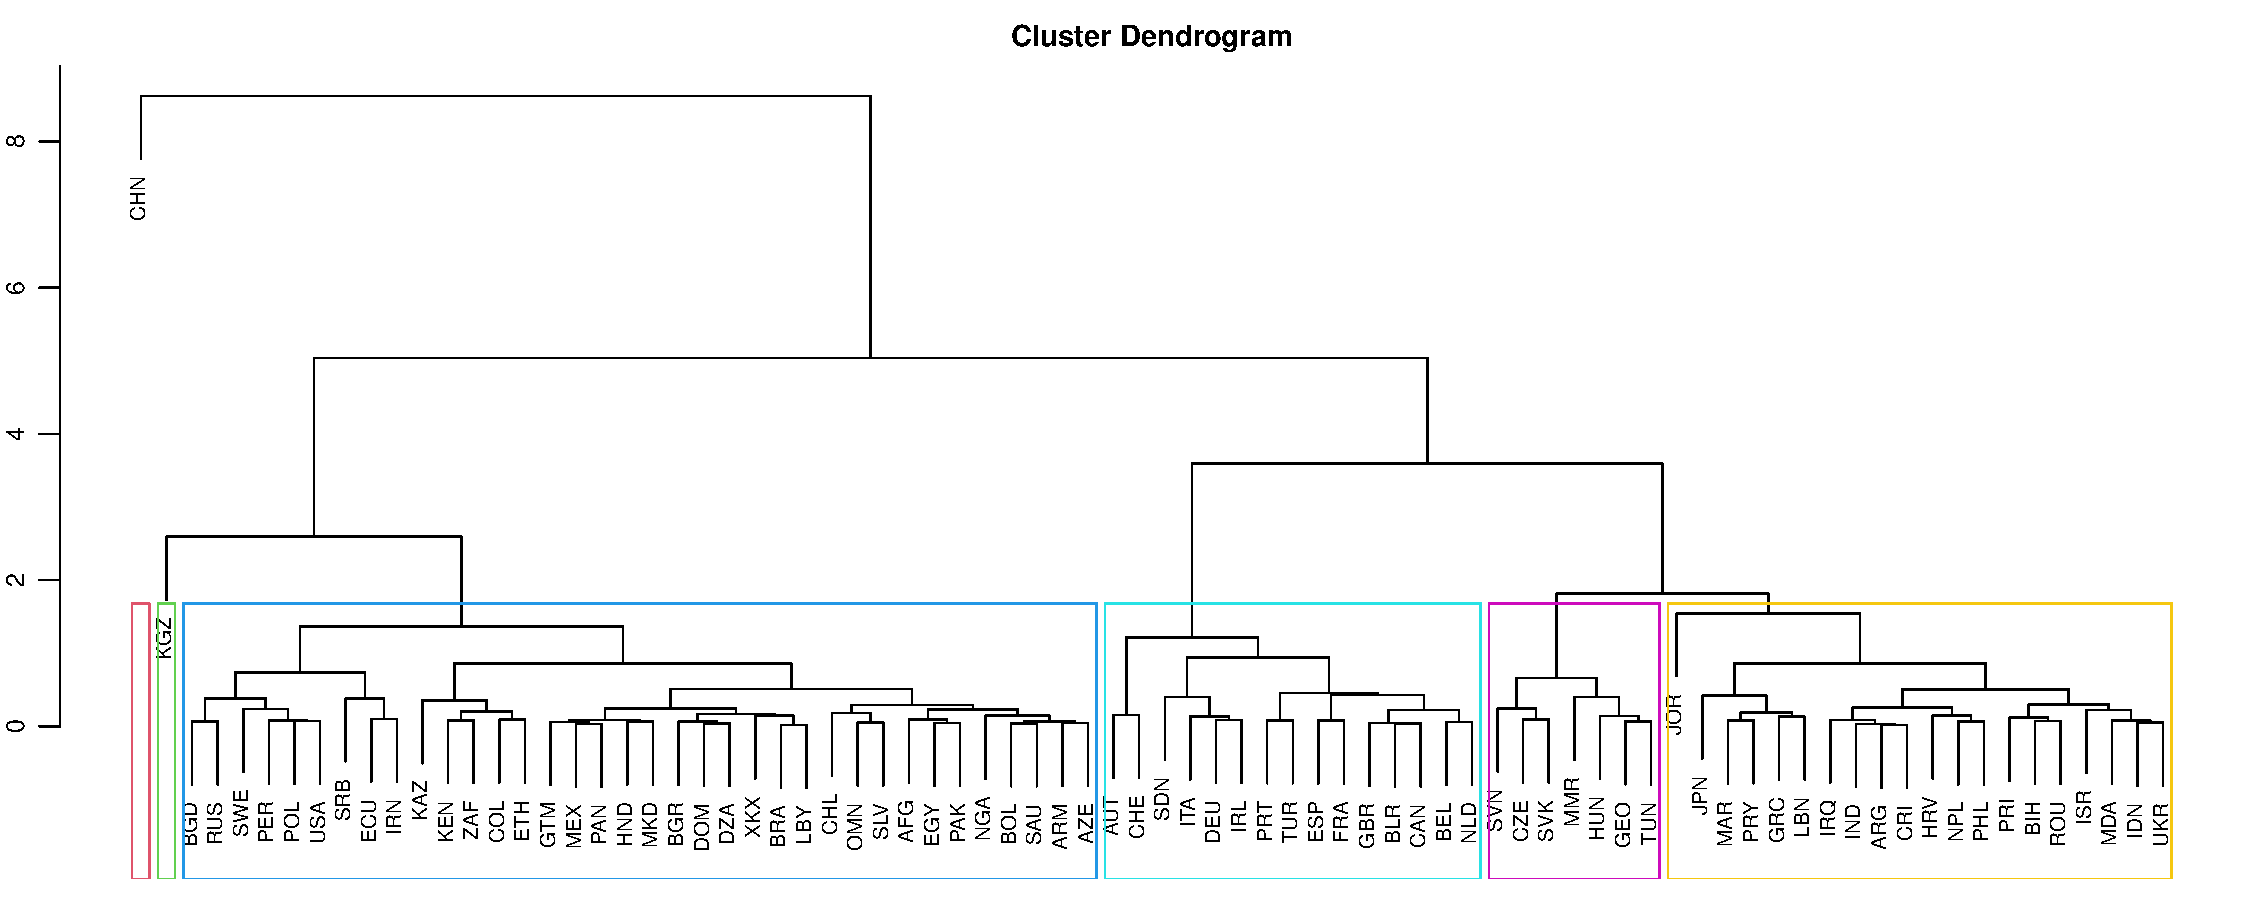
\includegraphics[width=\textwidth]{plots/dendrogram}
\caption{Results of HAC.}\label{fig:dend}
\end{minipage}
\end{figure}

\begin{figure}[t!]
\centering
\begin{subfigure}[b]{0.48\textwidth}
\subfloat[][]{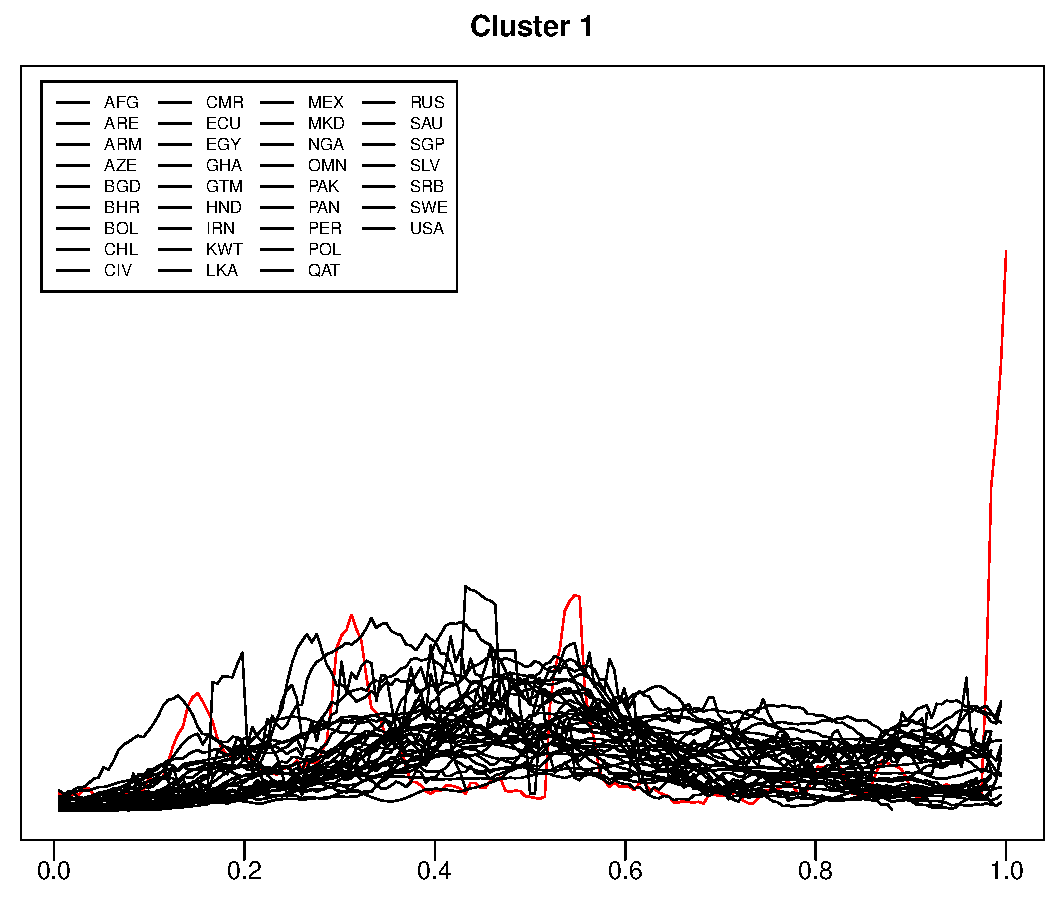
\includegraphics[width=\textwidth]{plots/results_cluster_1}\label{fig:cl1}}
\end{subfigure}\hspace{0.25cm}
\begin{subfigure}[b]{0.48\textwidth}
\subfloat[][]{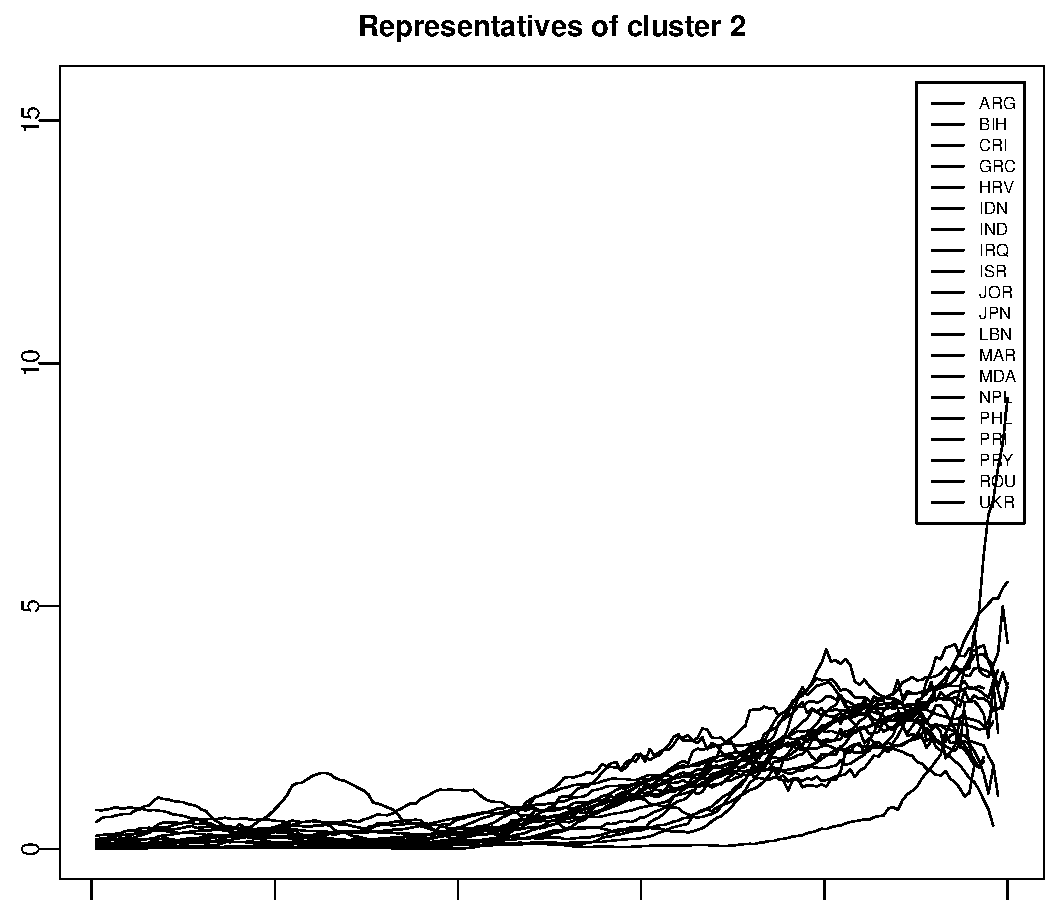
\includegraphics[width=\textwidth]{plots/results_cluster_2}\label{fig:cl2}}
\end{subfigure}\\
\begin{subfigure}[b]{0.48\textwidth}
\subfloat[][]{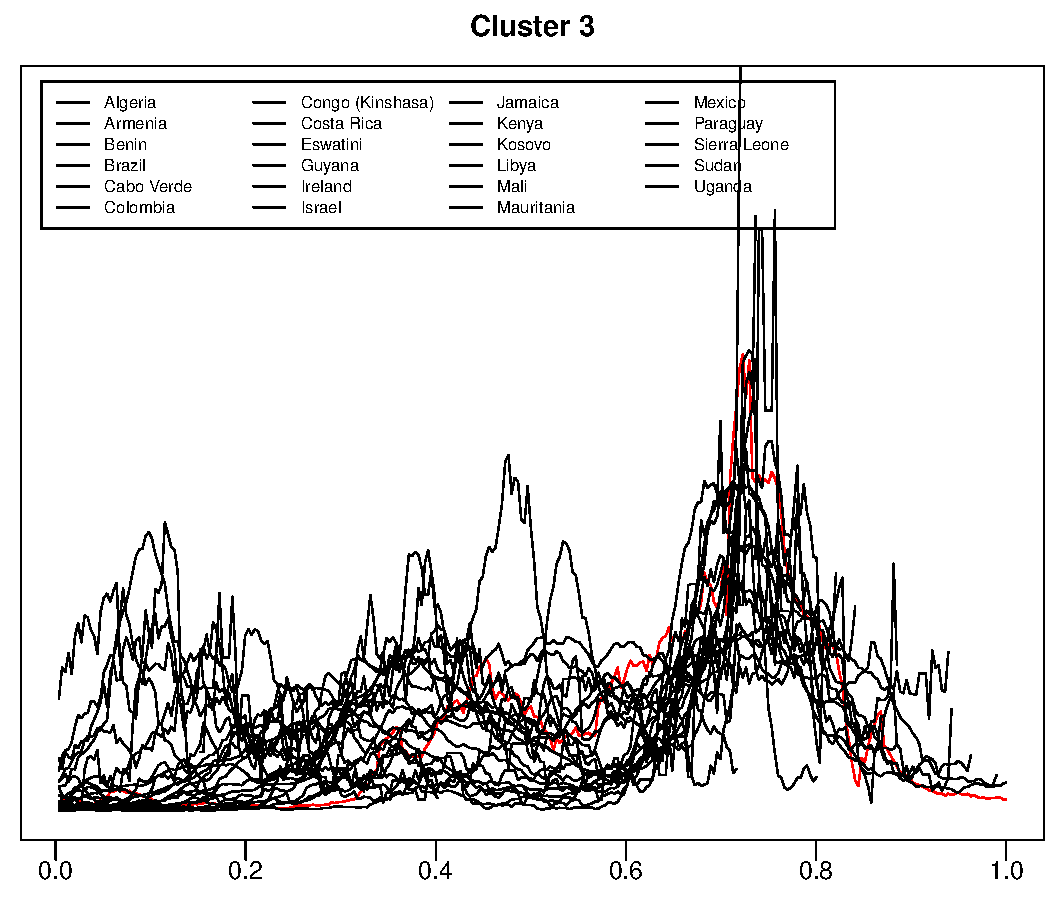
\includegraphics[width=\textwidth]{plots/results_cluster_3}\label{fig:cl3}}
\end{subfigure}\hspace{0.25cm}
\begin{subfigure}[b]{0.48\textwidth}
\subfloat[][]{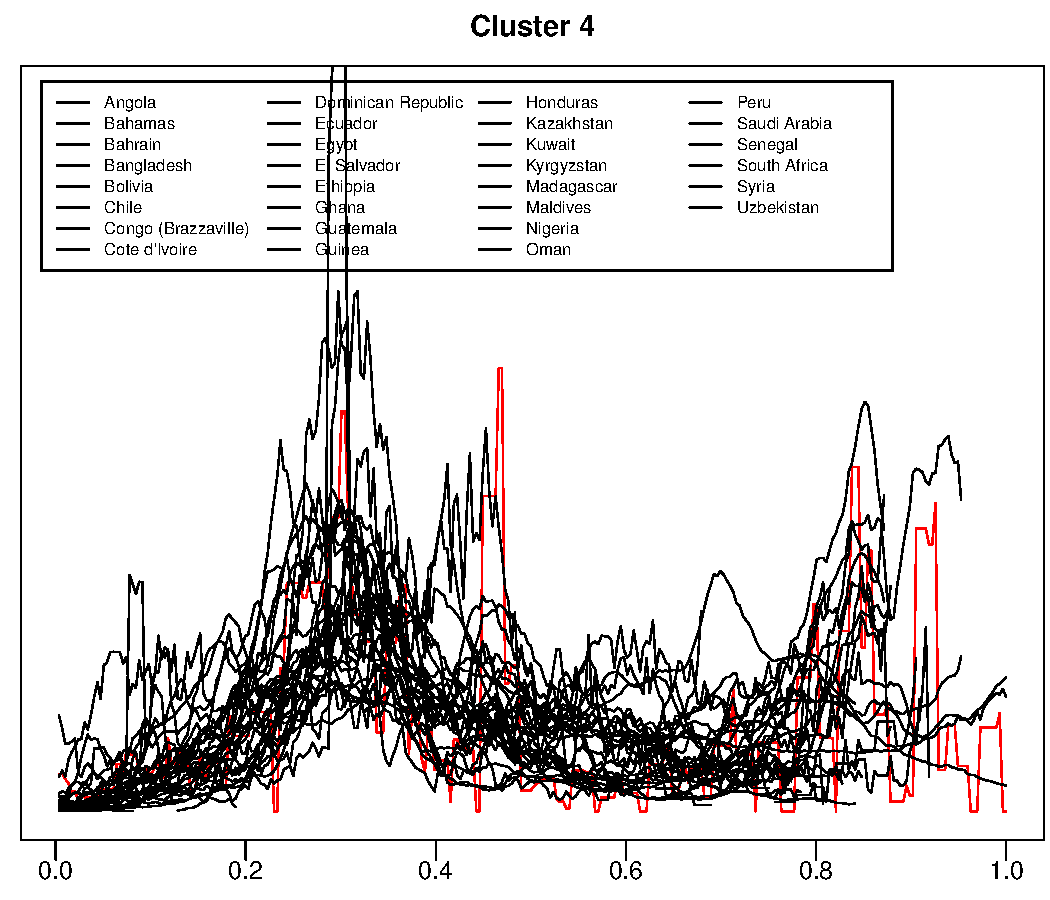
\includegraphics[width=\textwidth]{plots/results_cluster_4}\label{fig:cl4}}
\end{subfigure}\\
\begin{subfigure}[b]{0.48\textwidth}
\subfloat[][]{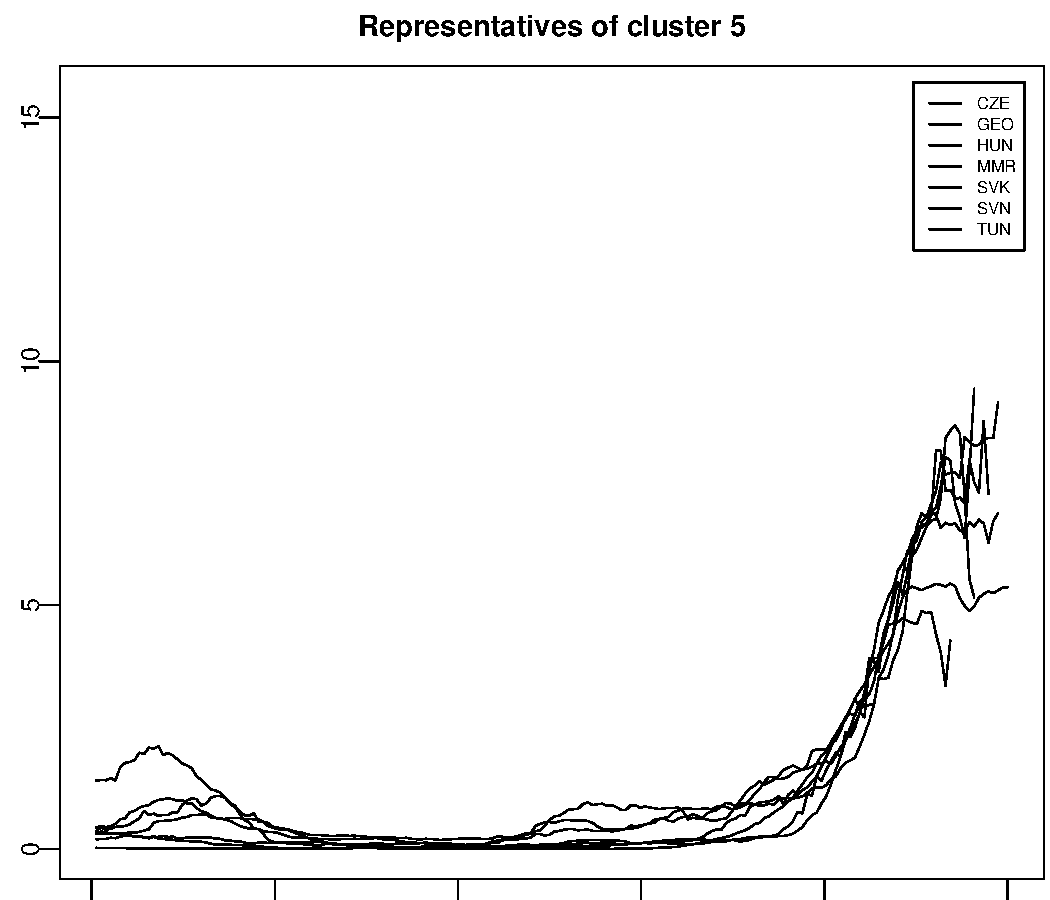
\includegraphics[width=\textwidth]{plots/results_cluster_5}\label{fig:cl5}}
\end{subfigure}\hspace{0.25cm}
\begin{subfigure}[b]{0.48\textwidth}
\subfloat[][]{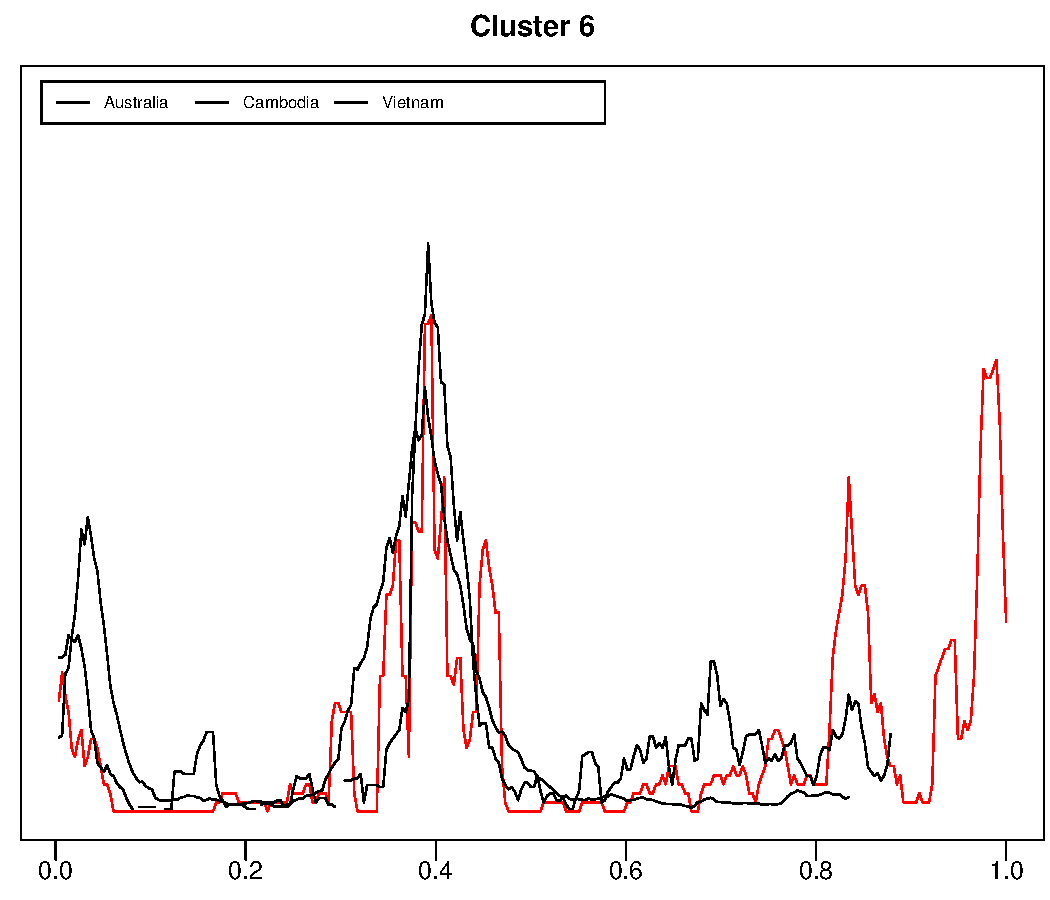
\includegraphics[width=\textwidth]{plots/results_cluster_6}\label{fig:cl6}}
\end{subfigure}
\end{figure}

\begin{figure}
\ContinuedFloat
\centering
\begin{subfigure}[b]{0.48\textwidth}
\subfloat[][]{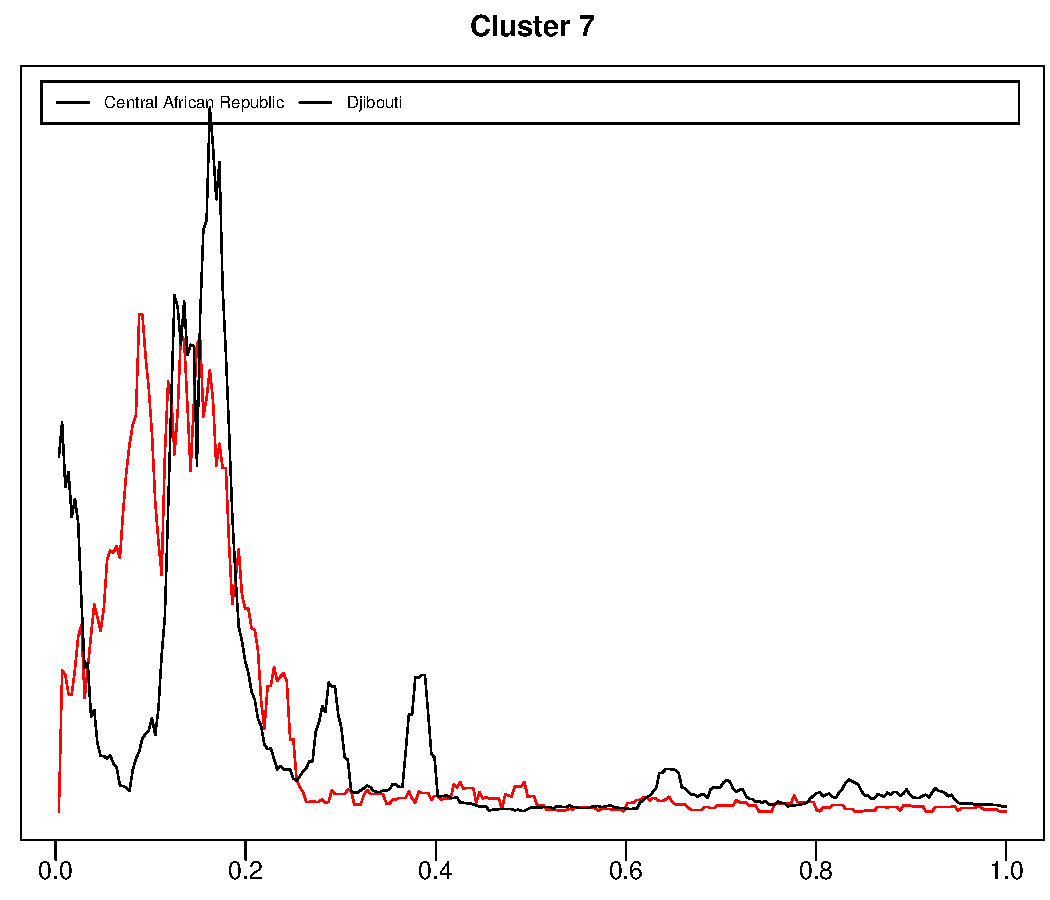
\includegraphics[width=\textwidth]{plots/results_cluster_7}\label{fig:cl7}}
\end{subfigure}
\caption{Clusters produced by the algorithm. Each panel presents appropriately scaled curve estimates $\widehat{m}_i$ that belong to a particular cluster.}\label{fig:clusters}
\end{figure}

\begin{figure}[t!]
\begin{minipage}[t]{0.98\textwidth}
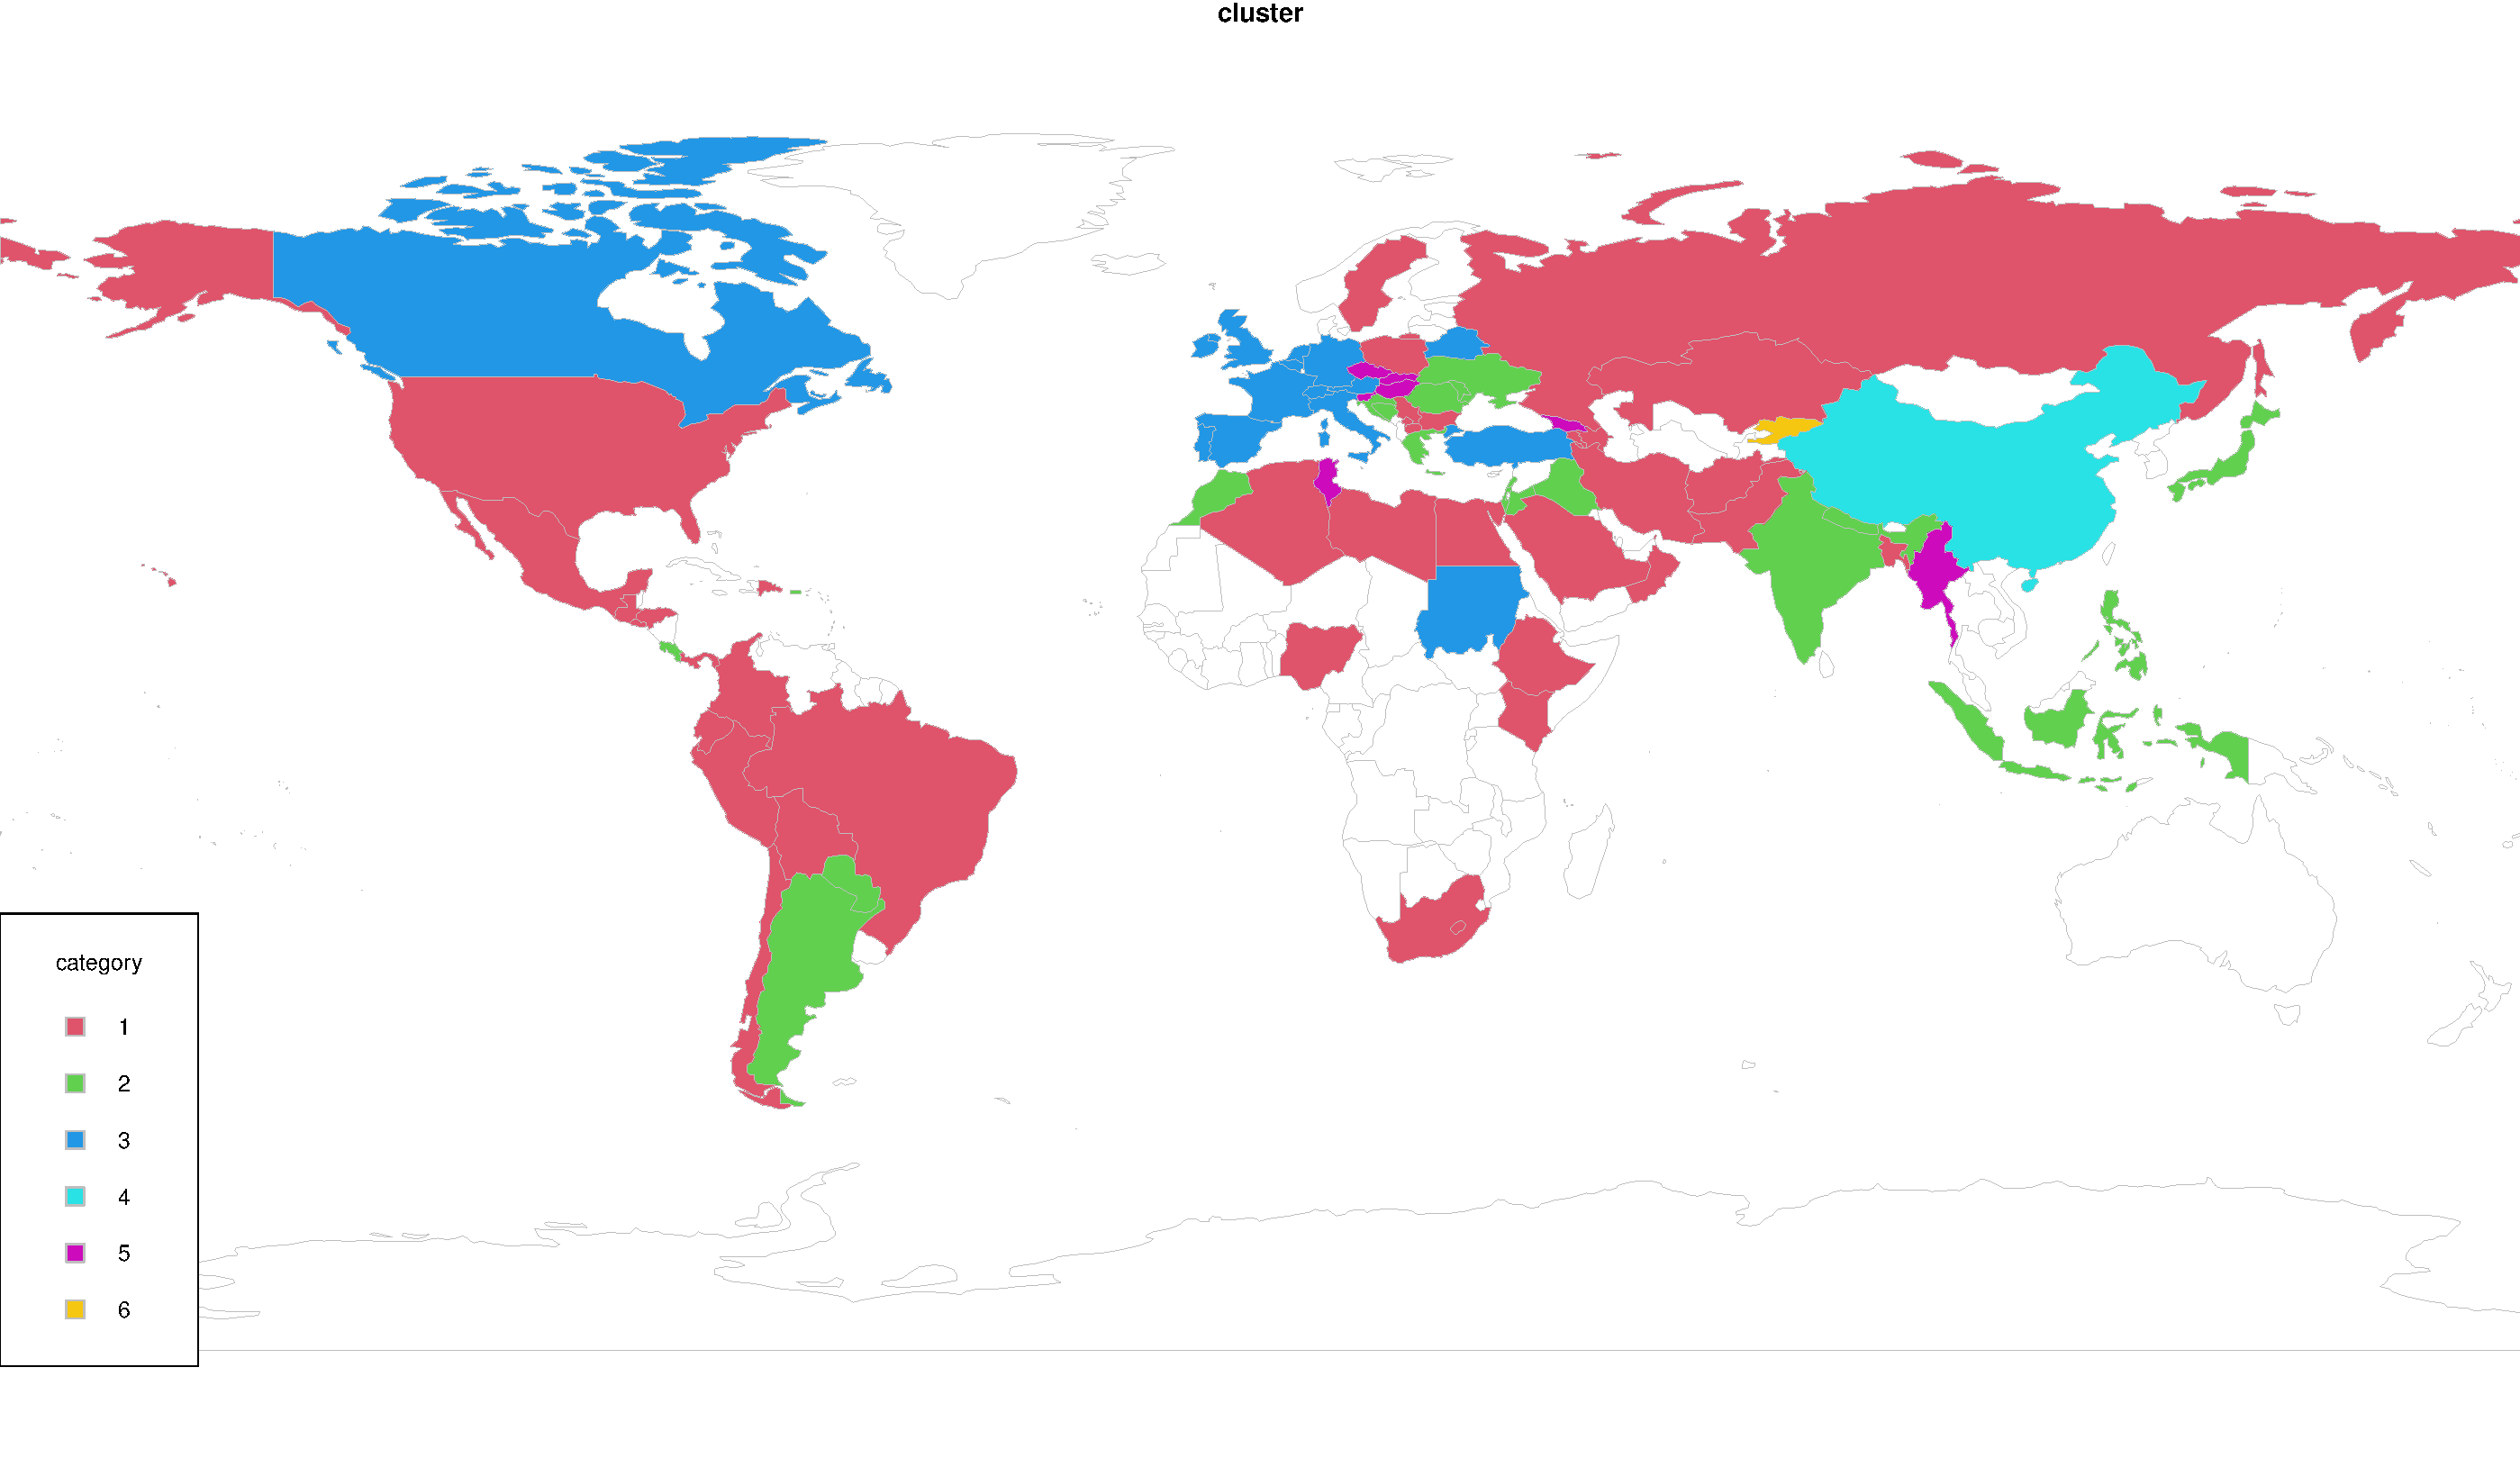
\includegraphics[width=\textwidth]{plots/choropleth}
\caption{Results of HAC on a map: each country is coloured according to the group it belongs to.}\label{fig:map}
\end{minipage}
\end{figure}


\clearpage
\bibliographystyle{ims}
{\small
\setlength{\bibsep}{0.35em}
\bibliography{bibliography}}



\end{document}
